\documentclass[a4paper, 12pt, reqno]{article}

\newcommand{\titl}{NumMeth MAT-410 Lab 2 Report}
\newcommand{\auth}{Moritz M. Konarski}
\usepackage{amsmath}
\usepackage{amssymb}
\usepackage[margin=0.95in]{geometry}
\usepackage[english]{babel}
\usepackage[pdftitle={\titl}, pdfauthor={\auth}, final]{hyperref}
\usepackage{graphicx}
\usepackage{mathptmx}
\usepackage[T1]{fontenc}
\usepackage{accents}
\usepackage{float}
\newcommand{\figref}[1]{Figure~\ref{#1}}
\newcommand{\tabref}[1]{Table~\ref{#1}}
\renewcommand{\baselinestretch}{1.2}
\setcounter{tocdepth}{2}
\usepackage{accents}
\usepackage[document]{ragged2e}

\setlength{\RaggedRightParindent}{0.25in}

\title{\titl}
\author{\auth}
\date{\today}

\begin{document}
\maketitle
\tableofcontents

\section{Introduction}

In this report I will detail my solutions to the tasks from our lab 2 PDF
regarding a weighted scheme for a one-dimensional heat equation.
I was assigned problem 4 and schemes 1, 2, and 3. For these schemes, I will
talk about the conditions for the Courant number and how to guarantee the
monotony of each of the schemes. Then the influence of monotony on the
correspondence of the numerical and analytic solutions will be discussed. The
possible deterioration in case monotony is not guaranteed will also be covered.
Finally, the three schemes will be compared with respect to their graphs and
errors for the same tasks.

\subsection{The Task}

The heat equation this report covers is the following:
\begin{equation}\nonumber
    \frac{\partial u}{\partial t} = \epsilon \frac{\partial^2 u}{\partial x^2} 
        + f(x,t); \qquad 0<x<1; \qquad t>0.
\end{equation}
The parameter $\epsilon$ lies on the interval $(0,1]$ and can be specified
using the parameter $k$ as $\epsilon = 2^{-k}$. In this report, $f(x,t) = 0$. 
The initial condition for this equation is
\begin{equation}\nonumber
    u(x,0) = \phi(x), \qquad 0 \le x \le 1
\end{equation}
and the boundary conditions are
\begin{equation}\nonumber
    \begin{gathered}
        u(0,t) = \psi_0(t),\\
        u(1,t) = \psi_1(t),\qquad t \ge 0.
    \end{gathered}
\end{equation}
This equation has both $x$ and $t$ as parameters, meaning that it changes in
$x$ and in time $t$.\\
The problem I am working with is problem 4 from our lab 2 PDF. It has two
additional parameters, $T1$ and $T2$, which are the initial temperatures on the
intervals $[0,0.5)$ and $(0.5, 1]$ respectively. At the point $x=0.5$, the
temperature equals $\frac{T1 + T2}{2}$.

\subsection{The Schemes}

This report covers 3 schemes, schemes 1, 2, and 3 from the lab 2 PDF. The
schemes are different ways of solving the above equation by first discretizing
the domain of $x$ and $t$ into grid points. The step size in $x$ is called $h$
and the step size in $t$ is called $\tau$. The equation is solved by iteration
through $t$ from $0$ to $t_{max}$ and for each $t_m$ by solving a system of
equations from $x=0$ to $x=1$. Then the weighted scheme (V.2.4)
from page 2 of lab 2 PDF gives this system of equations. (V.2.4) can be
transformed into a form (V.2.8) that can easily be solved using the tridiagonal
matrix algorithm (progonka). (V.2.8) is the formula for this algorithm
\begin{equation}\nonumber
    -Au^m_{i-1} + Bu_i^m - Cu^m_{i+1} = 
        A^0u^{m-1}_{i-1} + B^0u_i^{m-1} + C^0u^{m-1}_{i+1}.
\end{equation}
The parameters for this algorithm are defined in (V.2.9)--(V.2.11). (V.2.11)
contains the definition of the parameters in the equation above. They are
defined as
\begin{equation}\nonumber
    \begin{cases}
        A = C = \theta \cdot K, \\
        B = 1 + A + C,\\
        A^0 = C^0 = (1-\theta) \cdot K, \\
        B^0 = 1 - A^0 - c^0, \\
        K = \frac{\epsilon \tau}{h^2}.
    \end{cases}
\end{equation}
Here $K$ is the Courant number and $\theta$ (the "weight", $0 \le \theta \le 1$) is the parameter that
differentiates the schemes from each other. The following three schemes are
covered in this report:
\begin{enumerate}
    \item Explicit scheme (ES), where $\theta = 0$,
    \item Crank--Nicolson scheme (CNS), where $\theta = 0.5$,
    \item Implicit scheme (IS), where $\theta = 1$.
\end{enumerate}
The parameter $\theta$ dramatically changes the way these three schemes behave,
as will be demonstrated in the following sections.

\section{Monotonicity}

All three schemes are considered monotonous if the following conditions holds
(V.2.13)
\begin{equation}\nonumber
    \text{max}\left(0, 1-\frac{1}{2K}\right) \le \theta \le 1.
\end{equation}
In effect this means that for these schemes $K$ can only have values such that
$K \le 0.5$ or $K \le \frac{1}{2(1-\theta)}$.

\subsection{Explicit Scheme}

For this scheme $\theta = 0$, so
\begin{equation}\nonumber
    K \le \frac{1}{2(1-\theta)}; \quad
    K \le \frac{1}{2(1)}; \quad
    K \le 0.5.
\end{equation}
If $K \le 0.5$, ES is monotonous.

\subsection{Crank--Nicolson Scheme}

For this scheme $\theta = 0.5$, so
\begin{equation}\nonumber
    K \le \frac{1}{2(1-\theta)}; \quad
    K \le \frac{1}{2(0.5)}; \quad
    K \le 1.
\end{equation}
If $K \le 1$, CNS is monotonous.

\subsection{Implicit Scheme}

For this scheme $\theta = 1$, so
\begin{equation}\nonumber
    K \le \frac{1}{2(1-1)}; \quad
    K \le \frac{1}{2(0)}.
\end{equation}
Here, the limit of $K$ cannot be found, so I would say that IS is monotonous
for all $K$.

\section{Monotonicity and Accuracy}

Monotonicity has a positive influence on the accuracy of an approximation
because it tends to prohibit oscillations in the numerical solution.
Nonetheless, it is not a guarantee for accuracy. As an example of this,
consider the case where $T1=-2$, $T2=2$, $N=65$ (number of nodes in space),
$M=257$ (number of nodes in time), $\epsilon = 0.125$, and $t_{max} = 7$.\\
Using the formula laid out above, we can find $K$ to be equal to 14. This means
that both ES and CNS are not monotonous. For ES the numerical solution break
down completely, starts to oscillate, and the error becomes so large that the 
variable holding it overflows -- this would be the expected outcome. For CNS
however, which is also not monotonous, this is not the case. CNS only slightly
oscillates but converges to the analytic solution. This behavior can be seen in
\figref{ma01}.
\begin{figure}[H]
    \center
    \includegraphics[width=\textwidth]{../data/guarantee correspondece/cn_0}
    \vspace{-20pt}
    \caption{CNS for the values stated above at $t = 0.0273$ while not
    monotonous}
    \label{ma01}
\end{figure}
As $t$ increases and the sharp transition between the temperature levels
becomes more smooth, the oscillations become smaller and finally stop.\\
IS does not have trouble with this example because it is monotonous for any
value of $K$. \figref{ma02} compares the error of CNS and IS for this example
as $t$ progresses.
\begin{figure}[H]
    \center
    \fbox{\includegraphics[width=\textwidth]{../data/guarantee correspondece/err}}
    \vspace{-20pt}
    \caption{CNS and IS errors over time with a $\log_{10}$ $y$ axis}
    \label{ma02}
\end{figure}
We can see that IS starts out with a lower error but soon CNS becomes more
accurate because it is a generally more accurate method. The fact that it is
not monotonous makes it less accurate at the start but as soon as the function
becomes less extreme and easier to approximate CNS becomes more accurate.
This example illustrates that even if a scheme is not monotonous it can still
be accurate, maybe even more accurate than a monotonous scheme.\\
Monotonicity is a beneficial condition for a scheme and has a positive effect
on its accuracy. Nonetheless, the differences between schemes may have a larger
influence and a more accurate scheme might be able to overcome the
disadvantages of not being monotonous.

\section{Deterioration of Solutions}

A related question is whether a scheme that is not monotonous will deteriorate
over time, becoming less accurate as time goes on. If a scheme is not monotonous,
it might start to oscillate and deteriorate. To illustrate this point, I chose
$T1=-2$, $T2=2$, $t_{max}=7$, $\epsilon = 2^{-12}$, $N=65$, and $M=5$. This 
gives a Courant
number of $K=1.75$. Again, ES and CNS are not monotone and thus might
deteriorate.\\
Starting at $t=0$, all three schemes have the exact same shape, as see in
\figref{ds01}.
\begin{figure}[H]
    \center
    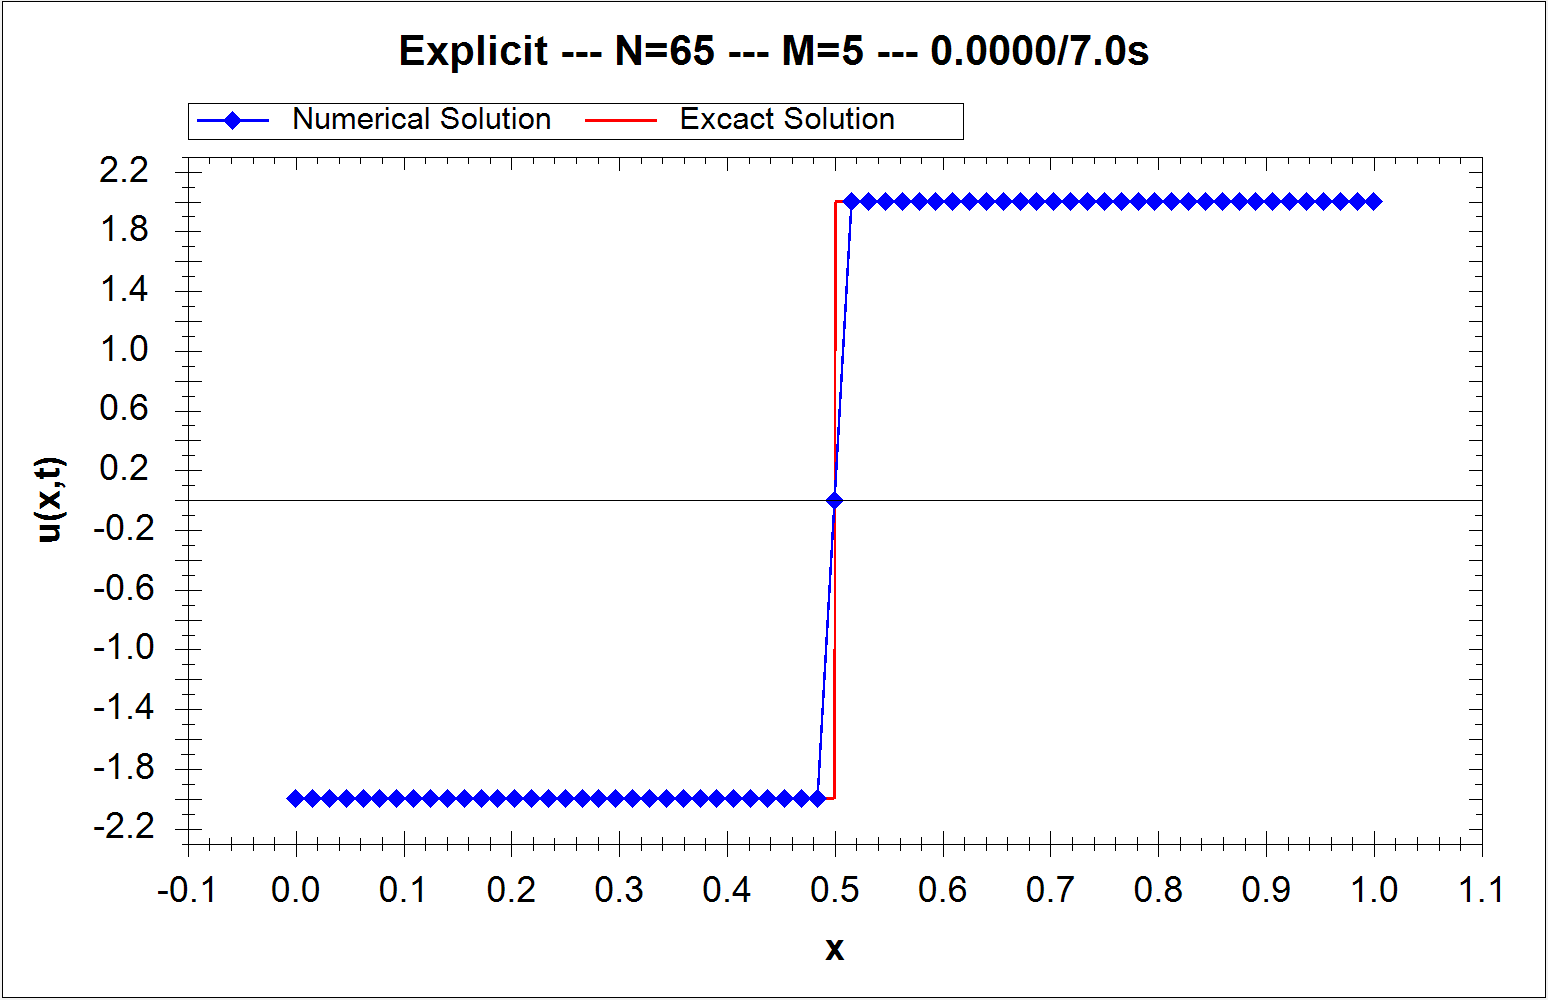
\includegraphics[width=\textwidth]{../data/not deterirated if not monotone/explicit_0}
    \vspace{-20pt}
    \caption{ES at $t=0$}
    \label{ds01}
\end{figure}
One time step further, ES has already started to strongly oscillate, see
\figref{ds02}.
\begin{figure}[H]
    \center
    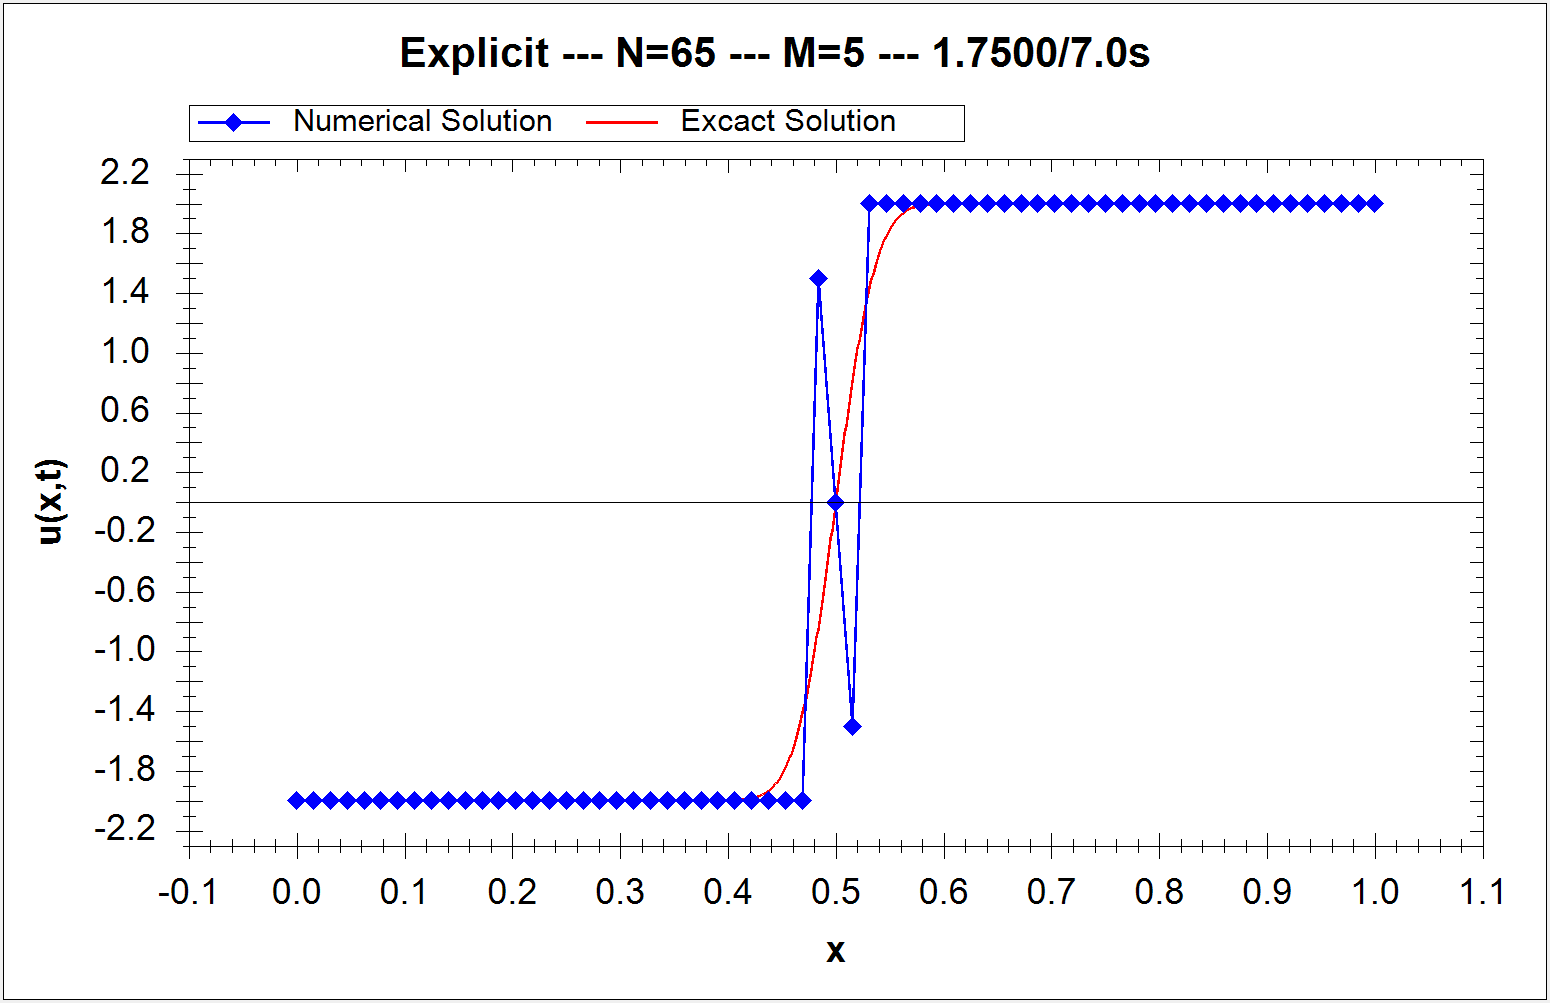
\includegraphics[width=\textwidth]{../data/not deterirated if not monotone/explicit_1}
    \vspace{-20pt}
    \caption{ES at $t=1.75$}
    \label{ds02}
\end{figure}
In contrast to this, the other scheme that is not monotone, CNS, does not
oscillate, see \figref{ds03}.
\begin{figure}[H]
    \center
    \includegraphics[width=\textwidth]{../data/not deterirated if not monotone/cn_0}
    \vspace{-20pt}
    \caption{CNS at $t=1.75$}
    \label{ds03}
\end{figure}
The behavior seen here continues for the whole time span of the analysis.
\figref{ds04} shows the errors of all three schemes for this problem.
\begin{figure}[H]
    \center
    \fbox{\includegraphics[width=\textwidth]{../data/not deterirated if not monotone/err}}
    \vspace{-20pt}
    \caption{ES, CNS, and IS errors over time}
    \label{ds04}
\end{figure}
It is obvious from \figref{ds04} that ES deteriorates and the error becomes
very large. CNS on the other hand remains accurate and does not deteriorate. In
\figref{ds05} the axis has been adjusted to show CNS and IS more clearly. The
same pattern as in the previous section emerges, as IS is more accurate for the
initial values of $t$ when the shape of the function is more extreme but then
CNS becomes more accurate as the functions smoothes out.
\begin{figure}[H]
    \center
    \fbox{\includegraphics[width=\textwidth]{../data/not deterirated if not monotone/err2}}
    \vspace{-20pt}
    \caption{ES, CNS, and IS errors over time; adjusted axis}
    \label{ds05}
\end{figure}
A non-monotonous scheme might deteriorate if it starts to oscillate strongly. ES
has shows that if it is not monotonous it will strongly oscillate and
deteriorate, while CNS,
despite not being monotonous, will not oscillate and thus it will not
deteriorate. IS is again not influenced by the monotonicity as it is always
monotonous.

\section{Comparison of the Schemes}

\subsection{Comparison 1}

To compare all 3 schemes in addition to the previous sections, I chose 2 more
illustrative examples. The first example has $N=5$, $M=5$, $T1=-2$, $T2=2$,
$\epsilon =1$, $t_{max}=1$, and a Courant number of $K=4$. Again, ES and CNS
are not monotonous. At $t=0$ all three
schemes look the same as shown here by IS in \figref{cs01}.
\begin{figure}[H]
    \center
    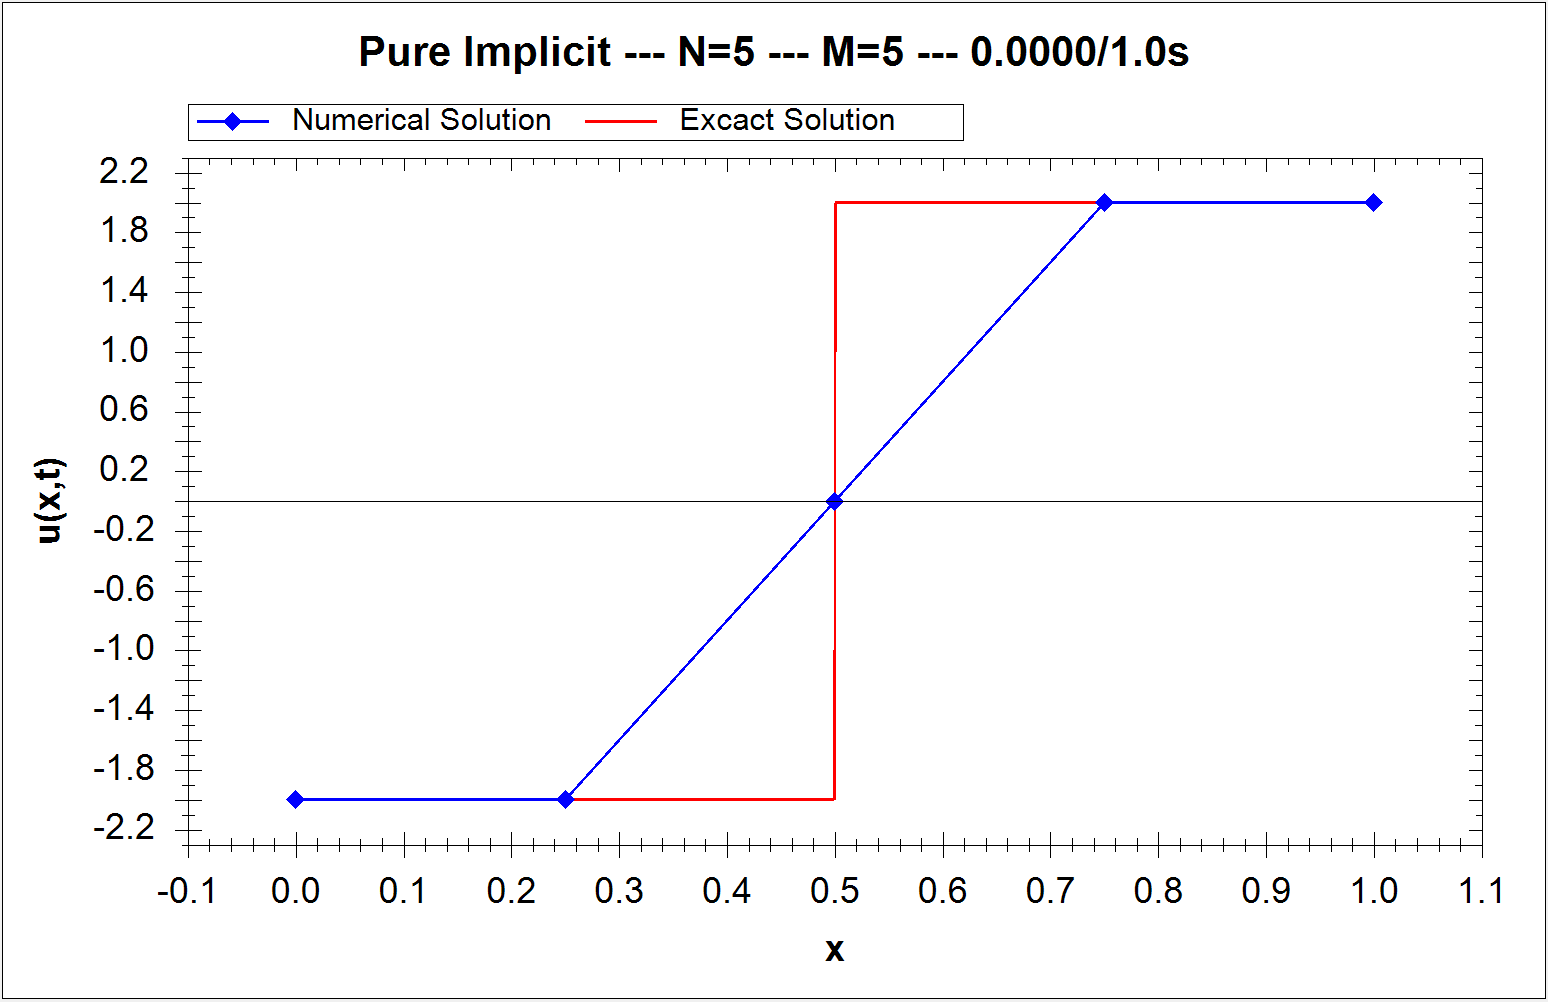
\includegraphics[width=\textwidth]{../data/comparison/1/e_0}
    \vspace{-20pt}
    \caption{IS at $t=0$}
    \label{cs01}
\end{figure}
In the next step, the differences between the schemes become obvious.
\figref{cs02} shows ES at $t=0.25$. We can see the oscillation and should take
note of the changed axis minimum and maximum in this graph.
\begin{figure}[H]
    \center
    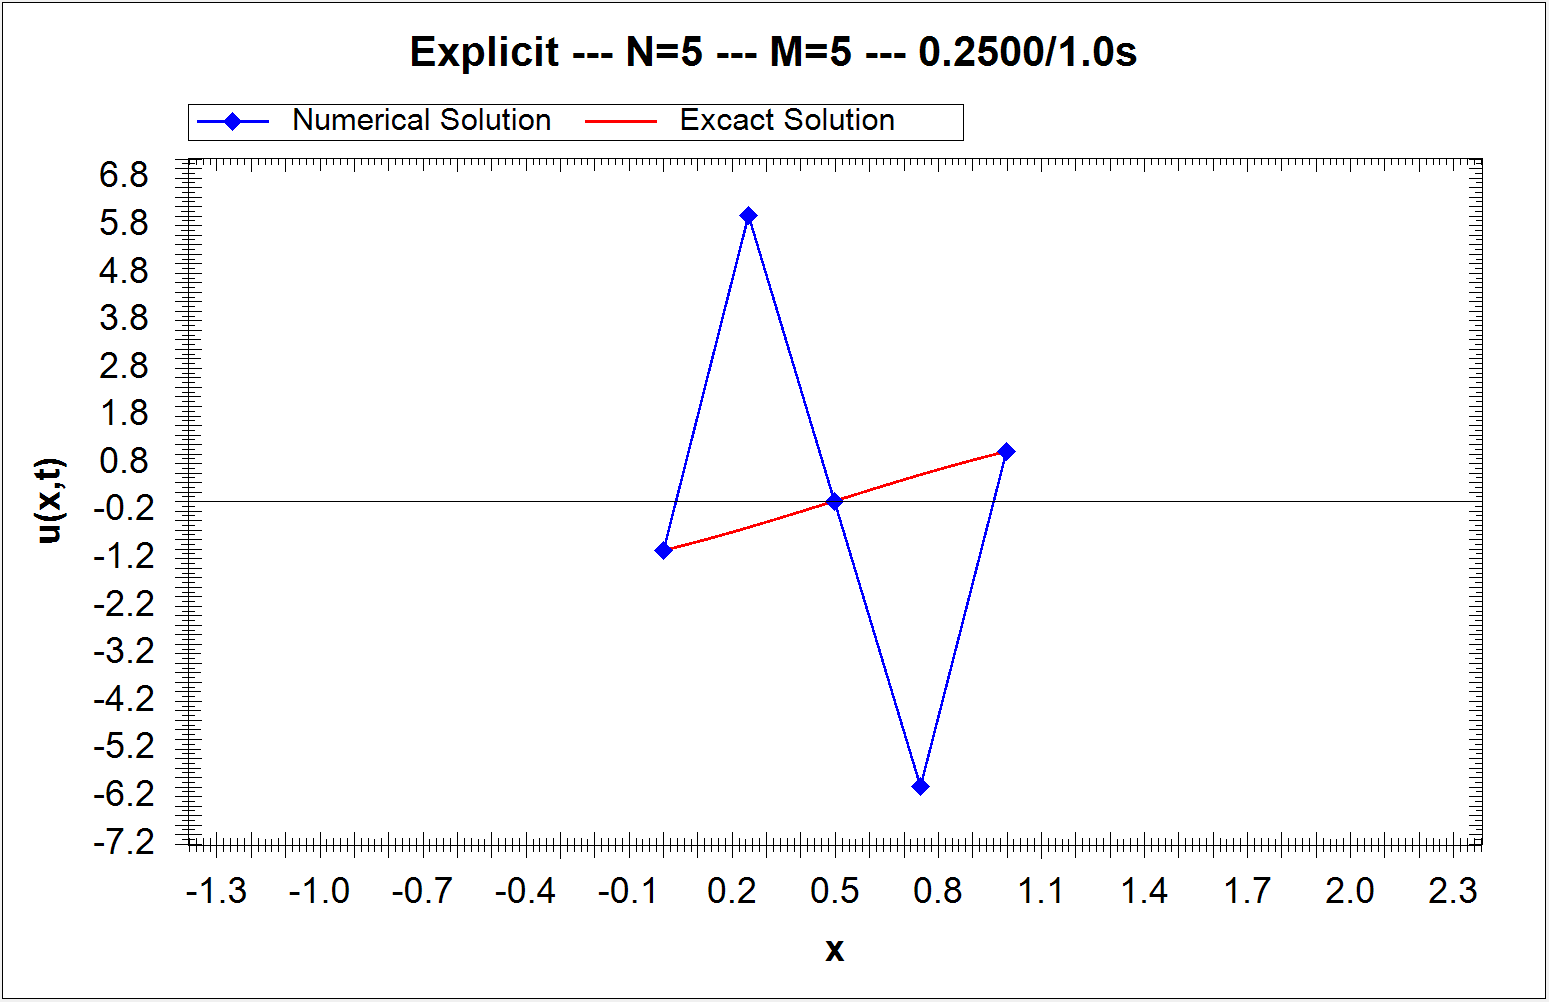
\includegraphics[width=\textwidth]{../data/comparison/1/ex_1}
    \vspace{-20pt}
    \caption{ES at $t=0.25$}
    \label{cs02}
\end{figure}
The behavior of CNS at the point $t=0.25$ is shown in \figref{cs03}.
\begin{figure}[H]
    \center
    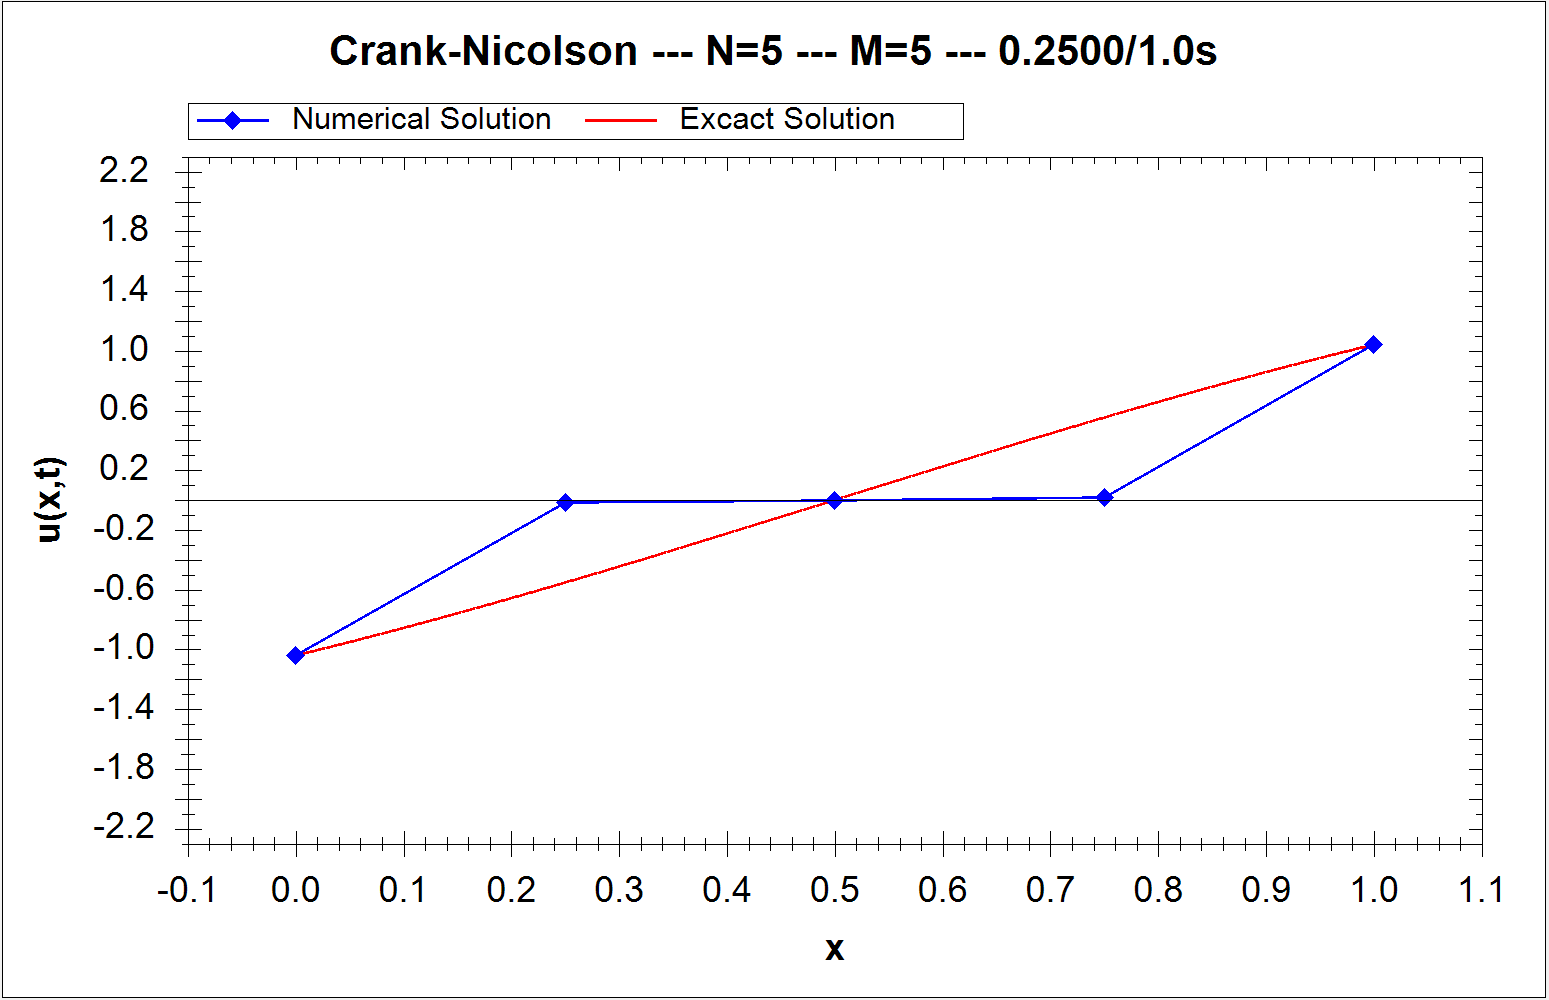
\includegraphics[width=\textwidth]{../data/comparison/1/cn_1}
    \vspace{-20pt}
    \caption{CNS at $t=0.25$}
    \label{cs03}
\end{figure}
Finally, IS at $t=0.25$ can be seen in \figref{cs04}.
\begin{figure}[H]
    \center
    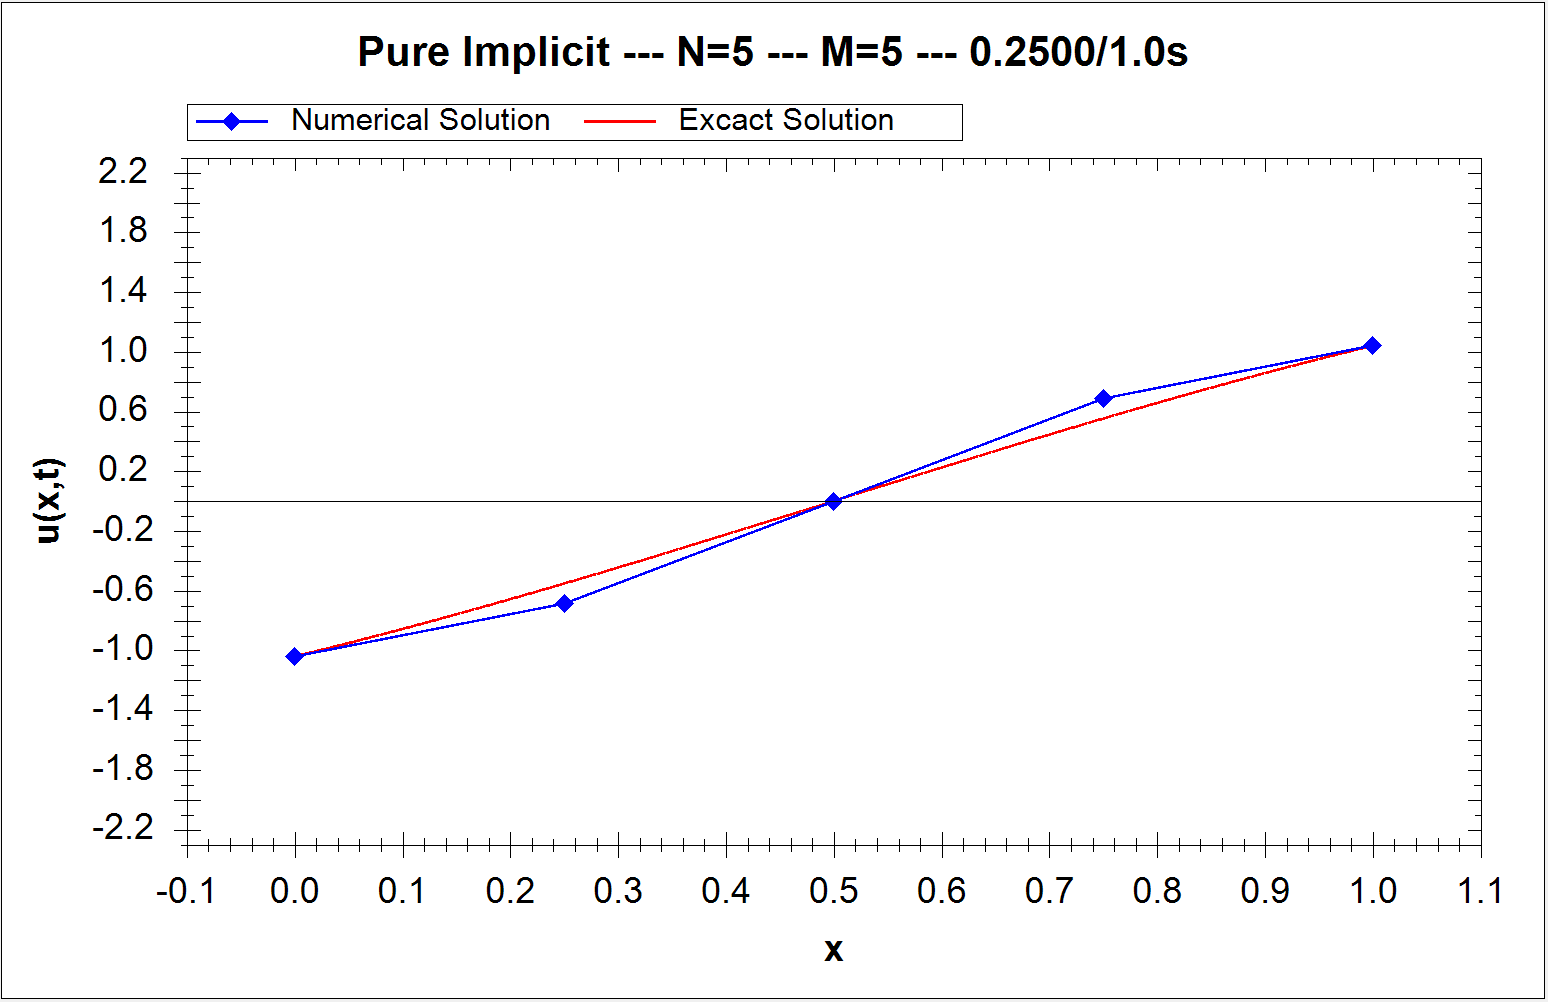
\includegraphics[width=\textwidth]{../data/comparison/1/e_1}
    \vspace{-20pt}
    \caption{IS at $t=0.25$}
    \label{cs04}
\end{figure}
These three figures support the assumption we have made previously that ES
oscillates and deteriorates when it is not monotonous and that CNS is more accurate 
even when not monotonous. Furthermore, IS is again the most accurate scheme 
when the shape of
the function is more extreme. \figref{cs05} shows the graphs of the errors and
summarizes these observations. A difference here is that IS remains the most
accurate scheme even as $t$ increases.
\begin{figure}[H]
    \center
    \fbox{\includegraphics[width=\textwidth]{../data/comparison/1/err}}
    \vspace{-20pt}
    \caption{ES, CNS, and IS errors over time}
    \label{cs05}
\end{figure}
To see the behavior, \figref{cs06} has an adjusted $y$ axis.
\begin{figure}[H]
    \center
    \fbox{\includegraphics[width=\textwidth]{../data/comparison/1/err2}}
    \vspace{-20pt}
    \caption{ES, CNS, and IS errors over time; $y$ axis adjusted}
    \label{cs06}
\end{figure}

\subsection{Comparison 2}

As a second comparison I finally chose parameters such that all 3 schemes are
monotonous. Those parameters are $T1=-2$, $T2=2$, $t_{max}=8$, $\epsilon
= 2^{-9}$, $N=129$, $M=513$. The Courant number for this example is $K=0.5$,
which is just within the limits of ES. \figref{cs07} contains the errors of the
3 schemes plotted against the value of $t$ for which they were found.
\begin{figure}[H]
    \center
    \fbox{\includegraphics[width=\textwidth]{../data/comparison/2/err}}
    \vspace{-20pt}
    \caption{ES, CNS, and IS errors over time; $\log_{10}$ scale}
    \label{cs07}
\end{figure}
We can see that ES is the least accurate for all values of $t$, followed by IS.
The most accurate of the three schemes is CNS. This observation is compatible
with our previous observation.

\section{Conclusion}

Taking into account all previous sections, I think that the implicit scheme is
the most versatile of the three schemes that I examined. It is monotonous for
all possible values which sets it apart from the other schemes. Being
unconditionally monotonous is an advantage because it prevents oscillations
from deteriorating the scheme's accuracy. The explicit scheme might be simple
and easy to compute, but it is not accurate enough to take advantage of that
(in my testing). While the implicit scheme is not
quite as accurate as the Crank--Nicolson scheme, it suffers fewer problems with
very abrupt changes in functions or monotonicity -- in my opinion that gives it
an advantage. Especially if the function (or its parameters) one wishes to 
numerically approximate is not completely known or investigated, the implicit
scheme would make sure that the result would not be hurt by monotonicity or
other problems.

\end{document}
